\documentclass[10pt]{article}

% Essential packages
\usepackage[utf8]{inputenc}
\usepackage[T1]{fontenc}
\usepackage{mathptmx} % Times font
\usepackage{geometry}
\usepackage{graphicx}
\usepackage{xcolor}
\usepackage{titlesec}
\usepackage{authblk}
\usepackage{setspace}
\usepackage{caption}
\usepackage{hyperref}
\usepackage{amsmath}
\usepackage{amssymb}
\usepackage[breakable]{tcolorbox}
\usepackage{float}
\usepackage{booktabs}
\usepackage{array}

\graphicspath{{figures/}}

% Page geometry - single column, comfortable margins
\geometry{letterpaper, top=2.5cm, bottom=2.5cm, left=2.5cm, right=2.5cm}

\hypersetup{colorlinks=true, linkcolor=blue, citecolor=blue, urlcolor=blue}

% Boxes
\newtcolorbox{methodbox}{
    colback=gray!10!white, colframe=gray!60!black,
    fonttitle=\bfseries\small, coltitle=black,
    boxrule=0.5pt, arc=2pt, left=3pt, right=3pt, top=3pt, bottom=3pt, breakable
}
\newtcolorbox{resultbox}{
    colback=green!5!white, colframe=green!60!black,
    fonttitle=\bfseries\small, coltitle=black,
    boxrule=0.5pt, arc=2pt, left=3pt, right=3pt, top=3pt, bottom=3pt, breakable
}

% Section formatting
\titleformat{\section}{\normalfont\fontsize{11}{13}\bfseries}{\thesection.}{0.5em}{}
\titlespacing*{\section}{0pt}{8pt}{4pt}
\titleformat{\subsection}{\normalfont\fontsize{10}{12}\bfseries\itshape}{\thesubsection}{0.5em}{}
\titlespacing*{\subsection}{0pt}{6pt}{3pt}

\captionsetup{font=small, labelfont=bf, format=plain, justification=justified,
              singlelinecheck=false, skip=5pt}

\setlength{\parindent}{0pt}
\setlength{\parskip}{4pt}
\setstretch{1.0}

\newcommand{\todo}[1]{{\color{red}[#1]}}

\author[1]{Eleni Nisioti}
\affil[1]{IT University of Copenhagen, Denmark}
\date{\today}

\title{\Large\bfseries Evolving Self-Replicating Digital Organisms:\\ An Experiment Summary}

\begin{document}
\maketitle

\begin{methodbox}
\textbf{Setup.} A JAX reimplementation of the self-replicating digital organisms of
Egri-Nagy \& Nehaniv (2003). Organisms are tapes occupying fixed cells on a
$128\times128$ toroidal grid ($16{,}384$ cells); they execute in place and reproduce
by writing a child into a neighbouring cell (OldestNurse placement). Each run is
seeded with $50$ copies of the hand-written \emph{arche.replicator} placed at random
positions. We run $5$ independent seeds ($62$--$66$) for $200{,}000$ cycles, with
copy-mutation rate $0.03$, insertion/deletion rate $0.0013$, $32$ micro-ops per
instruction, and the fast-track cache disabled. Full population snapshots are dumped
every $1{,}000$ cycles. \textbf{The data below covers only the first $\sim$3{,}000
cycles (runs ongoing); figures regenerate via \texttt{docs/make\_figures.py}.}
Seeds are shown as separate lines throughout.
\end{methodbox}

%---------------------------------------------------------------
\section{Population dynamics}
Each run begins as $50$ founders on an otherwise empty grid and colonises the free
space, so the living population climbs toward the $16{,}384$-cell carrying capacity
(Fig.~\ref{fig:population}, left). At cycle $3{,}000$ the grid is still far from
saturated ($\sim$3{,}500--4{,}000 alive). Self-replicators are present from the
outset and increase steadily (centre), and the number of reproduction events per
cycle grows with the population (right). The five seeds behave consistently,
differing mainly in colonisation speed --- a consequence of the random founder
placement.

\begin{figure}[H]
\centering
\begin{minipage}{0.87\textwidth}
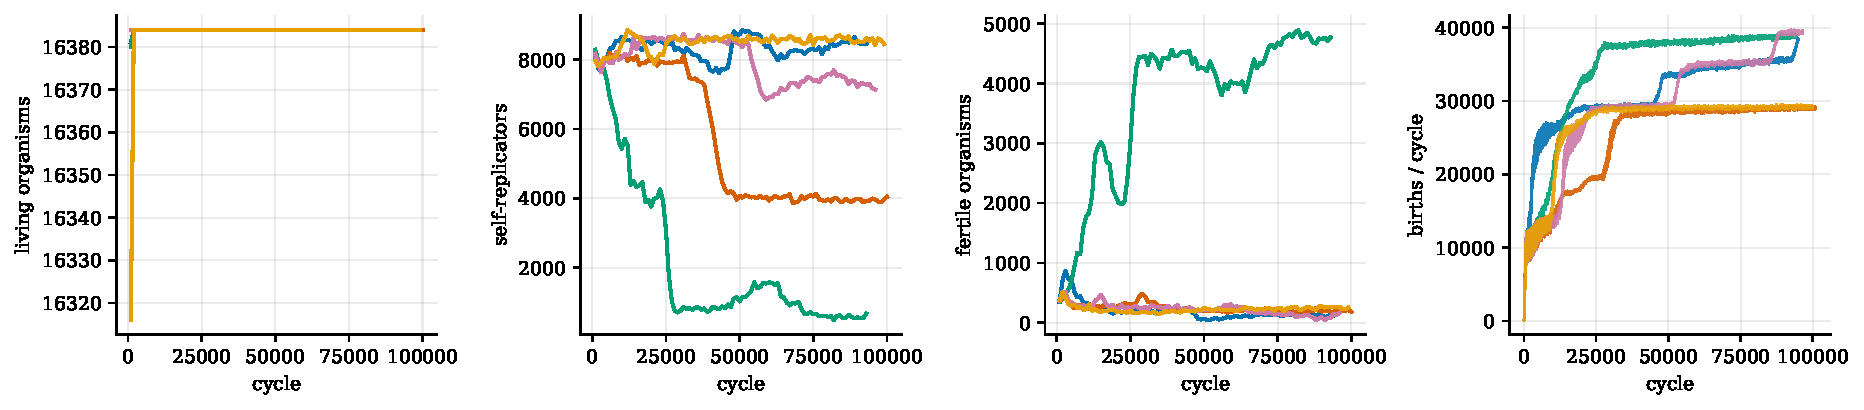
\includegraphics[width=\linewidth]{fig_population.pdf}
\end{minipage}\hfill
\begin{minipage}{0.11\textwidth}
\centering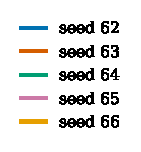
\includegraphics[width=\linewidth]{fig_legend.pdf}
\end{minipage}
\caption{\textbf{Population dynamics.} Living organisms, self-replicator count, and
births per cycle over time, for each of the five seeds. The population expands from
$50$ founders toward the grid capacity; self-replicators and births scale with it.}
\label{fig:population}
\end{figure}

%---------------------------------------------------------------
\section{Diversity: genomic and phenotypic}
We separate \emph{genomic} diversity (the genotype) from \emph{phenotypic} diversity,
and measure the phenotype at two levels --- the executable program and the resulting
behaviour --- each in its own panel (Fig.~\ref{fig:diversity}). The genomic panel
counts distinct \emph{raw genomes} among the self-replicators. The executable panel
resolves two sub-levels: distinct \emph{executed-token} sequences (the tape with junk /
non-executed positions dropped, but raw tokens kept) and distinct \emph{canonical-opcode}
programs (with synonymous encodings also collapsed). The gap between the raw genomes and
the executed tokens is non-coding junk; the (small) gap between executed tokens and
canonical opcodes is synonymous-encoding neutrality. The behavioural panel counts
distinct \emph{replication speeds} (distinct gestation times).

Diversity shrinks at each step of the genotype$\rightarrow$executable$\rightarrow$
behaviour map: genomic diversity far exceeds executed-token diversity --- most genetic
variation is in tape the machine never runs --- collapsing synonymous encodings removes
little further, and behavioural diversity is narrower still, as different programs
converge on a small set of replication speeds.

\begin{figure}[H]
\centering
\begin{minipage}{0.87\textwidth}
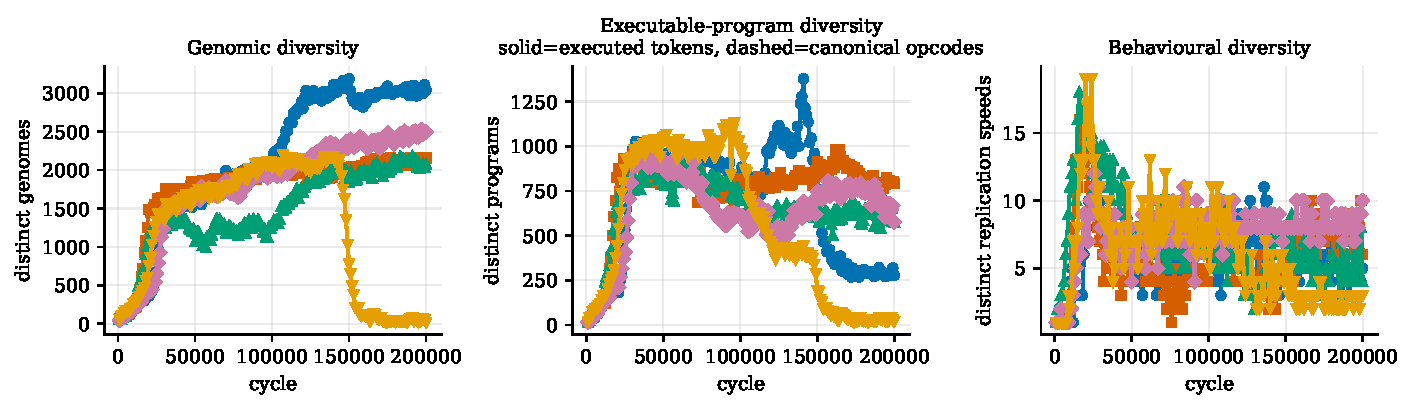
\includegraphics[width=\linewidth]{fig_diversity.pdf}
\end{minipage}\hfill
\begin{minipage}{0.11\textwidth}
\centering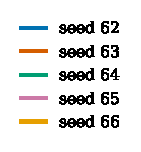
\includegraphics[width=\linewidth]{fig_legend.pdf}
\end{minipage}
\caption{\textbf{Diversity} of the self-replicators along the
genotype$\rightarrow$phenotype map. Left: distinct genomes (genotype). Centre:
distinct executable programs --- executed tokens with junk dropped (solid) vs.\
canonical opcodes with synonymous encodings also collapsed (dashed). Right: distinct
replication speeds (behavioural phenotype). Diversity decreases left to right.}
\label{fig:diversity}
\end{figure}

\begin{resultbox}
\textbf{Observation.} Genetic diversity substantially overstates functional
diversity: the collapse from raw to effective programs indicates that much of the
variation among self-replicators is neutral (junk / non-executed tape), while the
replication phenotype stays convergent.
\end{resultbox}

%---------------------------------------------------------------
\section{Genome structure}
Each genome is divided by a \texttt{SEP} marker into a \emph{header} (which defines the
organism's registers and instruction set --- the genotype$\rightarrow$phenotype map)
and a \emph{code} section (the executable program that uses it). We track the mean
length of the instruction-set header and of the code section separately, together with
the number of registers organisms define (Fig.~\ref{fig:genome}). Early on these stay
close to the seeded ancestor (a large instruction-defining header, a short code
section, $\sim$4 registers); drift in these structural quantities as the population
diversifies is the signal to watch at later cycles.

\begin{figure}[H]
\centering
\begin{minipage}{0.87\textwidth}
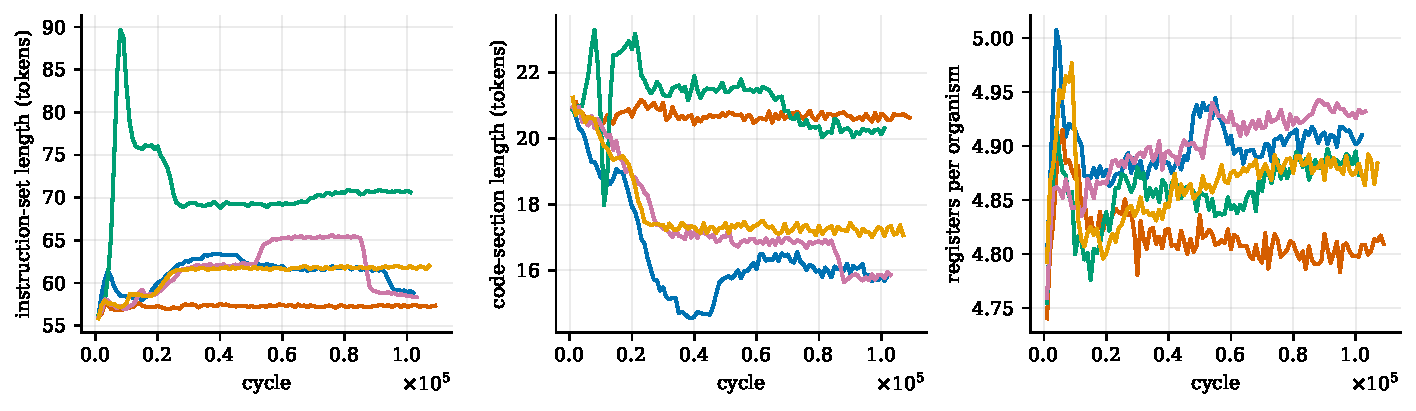
\includegraphics[width=\linewidth]{fig_genome.pdf}
\end{minipage}\hfill
\begin{minipage}{0.11\textwidth}
\centering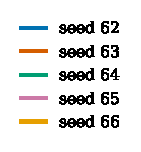
\includegraphics[width=\linewidth]{fig_legend.pdf}
\end{minipage}
\caption{\textbf{Genome structure.} Mean instruction-set (header) length, mean
code-section length, and mean number of registers per organism, each shown separately
and per seed.}
\label{fig:genome}
\end{figure}

%---------------------------------------------------------------
\section{Language}
Because each organism defines its own instruction set in its header, the population
develops a set of ``languages''. We summarise several properties.

\textbf{Entropy.} Several metrics are Shannon entropies (in nats). For a set of counts
$\{c_k\}$ over categories $k$ we form probabilities $p_k = c_k / \sum_j c_j$ and compute
\[
  H = -\sum_k p_k \ln p_k ,
\]
so $H = 0$ when a single category dominates and $H = \ln K$ (maximal) when all $K$
categories are equally frequent. We apply this at three levels: the pooled distribution
of raw opcode symbols across all genomes (\emph{symbol entropy}), the opcodes appearing
in the \emph{decoded instruction sets} (\emph{opcode entropy}), and the distribution of
distinct headers or ``dialects'' (\emph{dialect entropy}).

Fig.~\ref{fig:language} shows the \emph{coding fraction} (share of a genome's tokens
actually executed --- how much of the tape is functional) and the \emph{dialect entropy}
(how many self-defined languages coexist and how evenly). A rising coding fraction means
leaner genomes; a rising dialect entropy means the population is fragmenting into many
languages rather than converging on one.

\begin{figure}[H]
\centering
\begin{minipage}{0.80\textwidth}
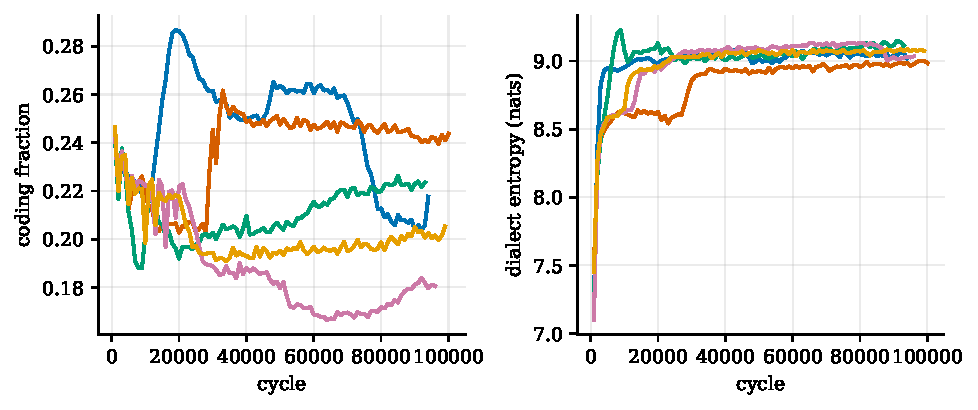
\includegraphics[width=\linewidth]{fig_language.pdf}
\end{minipage}\hfill
\begin{minipage}{0.13\textwidth}
\centering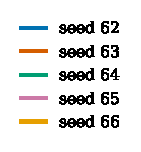
\includegraphics[width=\linewidth]{fig_legend.pdf}
\end{minipage}
\caption{\textbf{Language.} Left: coding fraction (executed share of the tape). Right:
dialect entropy (diversity of self-defined instruction sets). Shown per seed.}
\label{fig:language}
\end{figure}

We also track the make-up of the instruction sets (Fig.~\ref{fig:language2}). The
\emph{opcode vocabulary} is how many of the $44$ primitive opcodes are in use (currently
nearly all). \emph{Instructions defined vs.\ used} counts how many instructions each
organism declares against how many its program actually references; the gap is dead,
never-invoked code. Two further quantities are structural proxies for more complex
language properties. \emph{Instruction reuse} (recurrence) is the mean number of times
each used instruction is invoked by the program: a value above one means the program is
built by repeatedly calling a compact set of instructions rather than a flat,
use-once sequence. \emph{Instruction complexity} (a hierarchy proxy) is the mean number
of micro-ops bundled into each instruction --- the language has a genuine two-level
structure (micro-ops compose instructions, instructions compose the program), and this
measures how much is packaged at the instruction level. These are deliberately simple
proxies for compositionality and hierarchy; a fuller treatment (e.g.\ measuring
systematic genotype$\rightarrow$phenotype recombination) is left for future work.

\begin{figure}[H]
\centering
\begin{minipage}{0.72\textwidth}
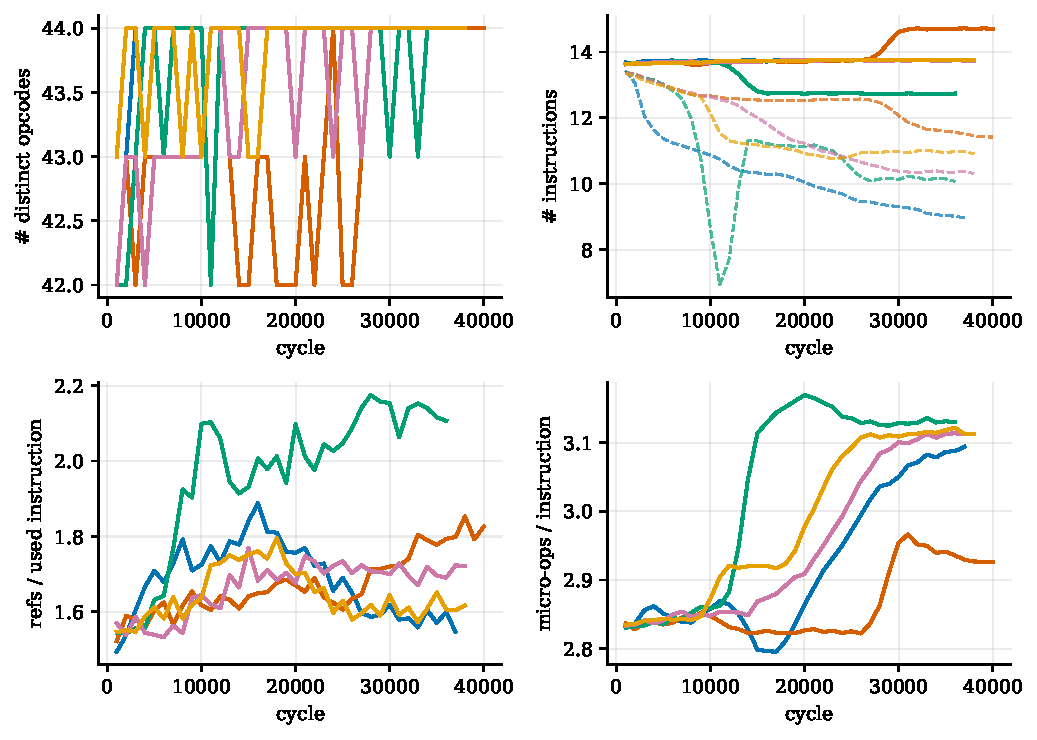
\includegraphics[width=\linewidth]{fig_language2.pdf}
\end{minipage}\hfill
\begin{minipage}{0.13\textwidth}
\centering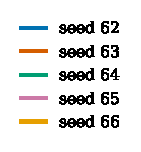
\includegraphics[width=\linewidth]{fig_legend.pdf}
\end{minipage}
\caption{\textbf{Language make-up.} Opcode vocabulary (distinct opcodes in use);
instructions defined (solid) vs.\ used (dashed); instruction reuse / recurrence (mean
invocations per used instruction); and instruction complexity / hierarchy (mean
micro-ops bundled per instruction). Per seed.}
\label{fig:language2}
\end{figure}

%---------------------------------------------------------------
\section{Genotype--phenotype map structure}
Beyond counting diversity we can look at the \emph{structure} of the
genotype$\rightarrow$phenotype map, in three complementary views (Fig.~\ref{fig:gpmap}).

The \emph{bipartite map} (left) makes the mapping explicit: one node per distinct
genotype and one per distinct phenotype (here the executable program), with an edge from
each genotype to the phenotype it expresses. Because the map is a function, a phenotype
node's degree equals its \emph{neutral-set size} --- how many genotypes map to it --- so
the large hubs are the highly redundant phenotypes. The distribution is strongly biased:
at cycle $6{,}000$ (seed~62) one phenotype gathers $25$ genotypes while most gather only
one or two.

The \emph{genotype network} (centre) instead connects genotypes to each other: nodes are
distinct genotypes, edges join those within one--two point-mutations/indels (so
mutationally related, recently-descended genotypes cluster), coloured by replication
speed. This asks whether genotypes sharing a phenotype form one connected \emph{neutral
network} or fragment into islands. Early on it is sparse and highly fragmented (the
dominant speed class splits into dozens of components), so self-replicator genotypes are
still mutationally spread out rather than forming a single connected neutral set.

Finally the \emph{redundancy} (right; no lineage and no mutations --- just grouping a
snapshot's genomes by phenotype) falls from $\sim$3.5 toward $\sim$2 as
executable-program diversity catches up with genomic diversity. Whether the neutral
islands coalesce as the population saturates is a key later-cycle question, connecting
directly to the paper's theme of the evolvability of the genotype--phenotype relation.

\begin{figure}[H]
\centering
\begin{minipage}{0.87\textwidth}
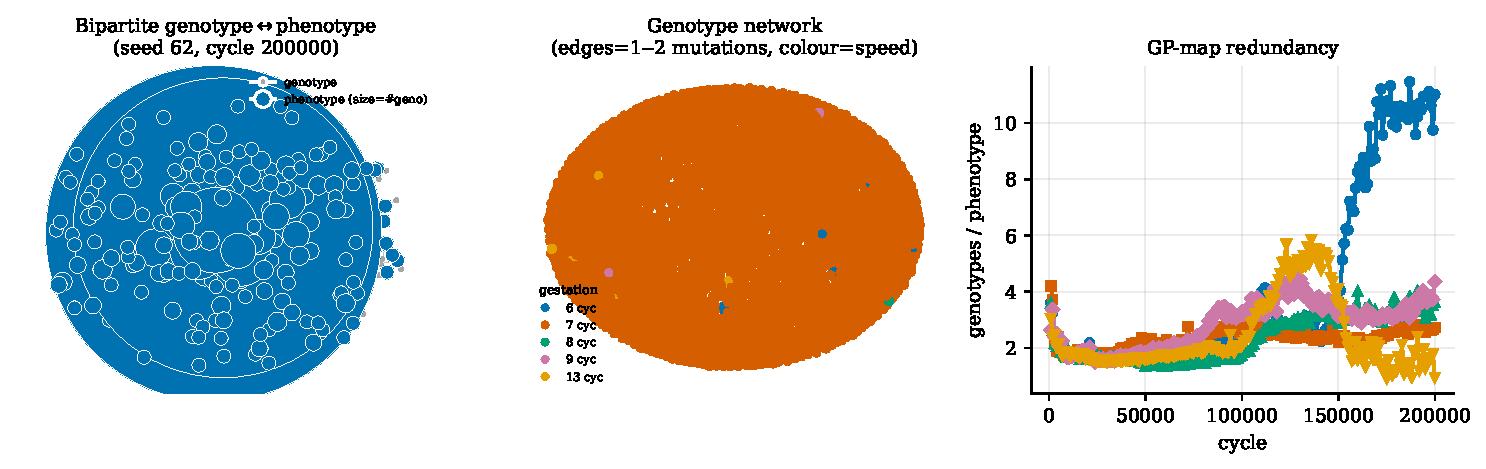
\includegraphics[width=\linewidth]{fig_gpmap.pdf}
\end{minipage}\hfill
\begin{minipage}{0.11\textwidth}
\centering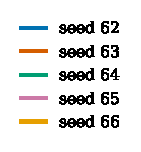
\includegraphics[width=\linewidth]{fig_legend.pdf}
\end{minipage}
\caption{\textbf{Genotype--phenotype map structure.} Left: bipartite map --- grey nodes
are genotypes, coloured nodes are phenotypes (executable programs) sized by how many
genotypes map to them. Centre: genotype network --- nodes are genotypes, edges join those
$1$--$2$ mutations apart, colour is replication speed; fragmented at this early stage.
Right: redundancy (genotypes per executable phenotype) over time, per seed. (The
seed-colour legend applies to the right panel only.)}
\label{fig:gpmap}
\end{figure}

\end{document}
